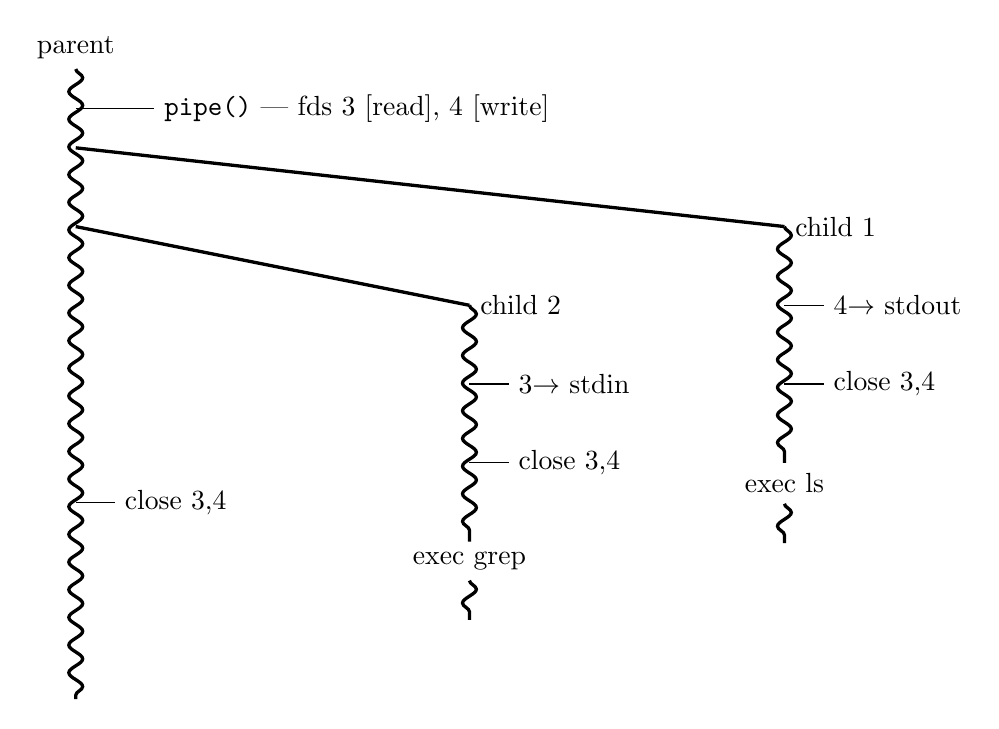
\begin{tikzpicture}
\tikzset{
    thread/.style={very thick,draw,decorate,decoration=snake},
    split/.style={very thick,draw},
    marker/.style={thin,draw},
}
\path[thread] (0, 0) --  (0, -8);
    \node[anchor=south] at (0,0) {parent};
\path[marker] (0, -.5) -- ++(1, 0) node[right] {\texttt{pipe()} --- fds 3 [read], 4 [write]};
    \path[split] (0, -1) --  (9, -2) node[right] {child 1};
    \path[marker] (9, -3) -- ++(.5, 0) node[right] {4$\rightarrow$ stdout};
    \path[marker] (9, -4) -- ++(.5, 0) node[right] {close 3,4};
    \path[thread] (9, -2) -- (9, -5) node[below] (exec ls) {exec ls};
    \path[thread] (exec ls.south) -- ++(0, -.5cm);

    \path[split] (0, -2) --  (5, -3) node[right] {child 2};
    \path[marker] (5, -4) -- ++(.5, 0) node[right] {3$\rightarrow$ stdin};
    \path[marker] (5, -5) -- ++(.5, 0) node[right] {close 3,4};
    \path[thread] (5, -3) -- (5, -6) node[below] (exec grep) {exec grep};
    \path[thread] (exec grep.south) -- ++(0, -.5cm);
    \path[marker] (0, -5.5) -- ++(.5, 0) node[right] {close 3,4};
\end{tikzpicture}